\documentclass{beamer}
\usetheme{Madrid}
\usecolortheme{whale}
\setbeamertemplate{navigation symbols}{}

% Packages
\usepackage{tikz}
\usepackage{booktabs}
\usepackage{amsmath}

% Title information
\title{Ethics and Race: Philosophical Perspectives}
\author{Brendan Shea, PhD}
\date{Introduction to Ethics}

\begin{document}
	
	\begin{frame}
	\titlepage
	\end{frame}
	
	
	% Slide 1: Introduction
	\begin{frame}
		\frametitle{Ethics and Race: Key Questions and Lesson Overview}
		
		\begin{itemize}
			\item This lesson examines the ethical dimensions of race through historical and philosophical lenses.
			\item We will analyze key arguments from W.E.B. Du Bois, Martin Luther King Jr., and Kwame Anthony Appiah.
			\item Throughout history, philosophers have engaged with questions of racial justice in different ways.
			\item These perspectives help us understand both historical contexts and contemporary ethical challenges.
		\end{itemize}
		
		\begin{alertblock}{Key Question}
			How have philosophical approaches to race evolved over time, and what ethical insights can we draw from them?
		\end{alertblock}
		
	\end{frame}
	
	% Slide 2: Philosophical Approaches
	\begin{frame}
		\frametitle{Philosophical Approaches to Race and Justice}
		
		\begin{itemize}
			\item \textbf{Ethics} is the systematic study of concepts of right and wrong conduct and the moral principles that govern behavior.
			\item Different philosophical traditions offer distinct frameworks for analyzing racial justice.
			\item These frameworks help us evaluate the moral arguments made throughout history regarding race.
			\item Understanding these approaches enables us to better analyze complex ethical questions.
		\end{itemize}
		
		\begin{block}{Major Philosophical Approaches}
			\begin{itemize}
				\item \textbf{Rights-Based}: Emphasizing inalienable human rights
				\item \textbf{Justice-Oriented}: Focused on fair distribution and treatment
				\item \textbf{Character-Focused}: Concerned with individual and societal virtue
				\item \textbf{Pragmatic}: Addressing practical social reform
			\end{itemize}
		\end{block}
		
	\end{frame}
	
	% Slide 3: Historical and Contemporary Perspectives
	\begin{frame}
		\frametitle{Historical and Contemporary Perspectives on Race and Ethics}
		
		\begin{itemize}
			\item Moral arguments about race have evolved significantly from the Revolutionary era to today.
			\item Historical contexts shaped how people understood and articulated ethical positions on race.
			\item Philosophical ideas have both reflected and challenged prevailing social attitudes about race.
			\item Contemporary discussions of race continue to engage with historical philosophical traditions.
		\end{itemize}
		
		\begin{center}
			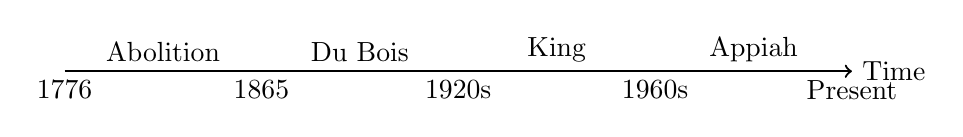
\begin{tikzpicture}
				\draw[->, thick] (0,0) -- (10,0) node[right] {Time};
				\node[below] at (0,0) {1776};
				\node[below] at (2.5,0) {1865};
				\node[below] at (5,0) {1920s};
				\node[below] at (7.5,0) {1960s};
				\node[below] at (10,0) {Present};
				\node[above] at (1.25,0) {Abolition};
				\node[above] at (3.75,0) {Du Bois};
				\node[above] at (6.25,0) {King};
				\node[above] at (8.75,0) {Appiah};
			\end{tikzpicture}
		\end{center}
		
	\end{frame}
	
	% Slide 4: American Revolution
	\begin{frame}
		\frametitle{The American Revolution: The Paradox of Liberty and Slavery}
		
		\begin{itemize}
			\item The American Revolution was founded on ideals of liberty and equality while maintaining slavery.
			\item \textbf{Natural rights philosophy} articulated by Jefferson claimed "all men are created equal" while excluding enslaved people.
			\item This fundamental contradiction created ethical tensions in American political thought.
			\item Early abolitionists used these same revolutionary principles to argue against slavery.
		\end{itemize}
		
		\begin{table}
			\begin{tabular}{ll}
				\toprule
				\textbf{Revolutionary Ideals} & \textbf{Contradictory Practices} \\
				\midrule
				Liberty for all & Enslavement of millions \\
				Natural rights & Legal denial of personhood \\
				Self-determination & Forced labor \\
				Equality & Racial hierarchy \\
				\bottomrule
			\end{tabular}
		\end{table}
		
	\end{frame}
	
	% Slide 5: Abolitionist Arguments
	\begin{frame}
		\frametitle{Abolitionist Moral Arguments Against Slavery}
		
		\begin{itemize}
			\item Abolitionists developed moral arguments grounded in religious and secular philosophical traditions.
			\item \textbf{Religious abolitionists} like Quakers argued that slavery violated divine law and Christian principles of human dignity.
			\item Secular abolitionists appealed to natural rights philosophy and the inconsistency of American ideals.
			\item Frederick Douglass emphasized how slavery corrupted both the enslaved and the enslaver's moral character.
		\end{itemize}
		
		\begin{exampleblock}{Frederick Douglass on Moral Corruption}
			"Slavery does away with fathers, as it does away with families. Slavery has no use for either fathers or families, and its laws do not recognize their existence in the social arrangements of the plantation."
		\end{exampleblock}
		
	\end{frame}
	
	% Slide 6: Pro-Slavery Arguments
	\begin{frame}
		\frametitle{Pro-Slavery Arguments: Examining Historical Justifications}
		
		\begin{itemize}
			\item Defenders of slavery developed complex ethical justifications for the institution.
			\item \textbf{Paternalism} claimed that slavery benefited enslaved people who were viewed as incapable of self-governance.
			\item Biblical arguments selectively used religious texts to justify racial hierarchy and slavery.
			\item Economic arguments claimed that slavery was necessary for prosperity and social order.
		\end{itemize}
		
		\begin{columns}
			\column{0.48\textwidth}
			\textbf{Religious Justifications}
			\begin{itemize}
				\item "Curse of Ham" narrative
				\item Divine ordering of society
				\item Enslavement in biblical texts
			\end{itemize}
			
			\column{0.48\textwidth}
			\textbf{Pseudo-Scientific Claims}
			\begin{itemize}
				\item Racial hierarchy theories
				\item Polygenesis (separate creation)
				\item Phrenology and cranial studies
			\end{itemize}
		\end{columns}
		
	\end{frame}
	
	% Slide 7: Ethical Crisis of the Union
	\begin{frame}
		\frametitle{The Ethical Crisis of the Union: Compromise vs. Moral Principle}
		
		\begin{itemize}
			\item The decades before the Civil War featured ethical debates about prioritizing national unity over moral principle.
			\item \textbf{Compromise} arguments claimed that preserving the Union justified tolerating slavery where it existed.
			\item Radical abolitionists rejected compromise, arguing that moral principles transcended political expediency.
			\item These debates highlighted tensions between pragmatic politics and moral absolutism.
		\end{itemize}
		
		\begin{block}{Lincoln's Evolving Position}
			Initially focused on preventing slavery's expansion while preserving the Union:
			\begin{quote}
				"If I could save the Union without freeing any slave I would do it, and if I could save it by freeing all the slaves I would do it; and if I could save it by freeing some and leaving others alone I would also do that."
			\end{quote}
			Later evolved toward emancipation as both moral necessity and military strategy.
		\end{block}
		
	\end{frame}
	
	% Slide 8: Emancipation and Reconstruction
	\begin{frame}
		\frametitle{Emancipation and Reconstruction: New Ethical Horizons}
		
		\begin{itemize}
			\item The Emancipation Proclamation (1863) and 13th Amendment (1865) legally ended slavery in the United States.
			\item Reconstruction introduced a new ethical framework of \textbf{citizenship rights} for formerly enslaved people.
			\item The 14th and 15th Amendments established legal equality and voting rights, transforming ethical discourse.
			\item This period raised fundamental questions about repair, restitution, and the meaning of freedom.
		\end{itemize}
		
	\end{frame}
	
	% Slide 9: The Rise of Jim Crow
	\begin{frame}
		\frametitle{The Rise of Jim Crow: Legalized Discrimination}
		
		\begin{itemize}
			\item Following Reconstruction, Southern states established \textbf{Jim Crow laws} to legally enforce racial segregation.
			\item The Supreme Court's Plessy v. Ferguson (1896) decision endorsed "separate but equal" segregation as constitutional.
			\item These laws created a comprehensive system of racial control backed by violence and intimidation.
			\item Jim Crow represented a moral regression, reestablishing racial hierarchy through new legal mechanisms.
		\end{itemize}
		
		\begin{alertblock}{Key Philosophical Question}
			How could a nation that had constitutionally established equal rights revert to a system of legal discrimination and disenfranchisement?
		\end{alertblock}
		
	\end{frame}
	
	% Slide 10: Resistance and Moral Arguments
	\begin{frame}
		\frametitle{Resistance and Moral Arguments Against Segregation}
		
		\begin{itemize}
			\item African Americans developed various forms of resistance to Jim Crow, each with distinct ethical justifications.
			\item \textbf{Accommodationism}, represented by Booker T. Washington, emphasized economic self-improvement and gradual progress.
			\item More radical approaches demanded immediate political rights and challenged the moral foundation of segregation.
			\item These divergent strategies reflected different ethical assessments of how to respond to injustice.
		\end{itemize}
		
		\begin{table}
			\scriptsize
			\begin{tabular}{lll}
				\toprule
				\textbf{Strategy} & \textbf{Key Figure} & \textbf{Ethical Emphasis} \\
				\midrule
				Accommodationism & Booker T. Washington & Virtue, self-improvement \\
				Political activism & W.E.B. Du Bois & Rights, dignity, justice \\
				Pan-Africanism & Marcus Garvey & Self-determination, pride \\
				Legal challenges & NAACP & Constitutional principles \\
				\bottomrule
			\end{tabular}
		\end{table}
		
	\end{frame}
	
	% Slide 11: W.E.B. Du Bois: Life and Context
	\begin{frame}
		\frametitle{W.E.B. Du Bois: Life, Education, and Historical Context}
		
		\begin{itemize}
			\item W.E.B. Du Bois (1868-1963) was born just after the Civil War and lived through Jim Crow, the Civil Rights Movement, and decolonization.
			\item As the first African American to earn a Ph.D. from Harvard (1895), Du Bois combined rigorous scholarship with activism.
			\item He conducted pioneering sociological research on Black communities, challenging prevailing racist assumptions.
			\item Du Bois co-founded the NAACP in 1909 to advance civil rights through legal challenges and public education.
		\end{itemize}
		
		\begin{center}
			\scriptsize
			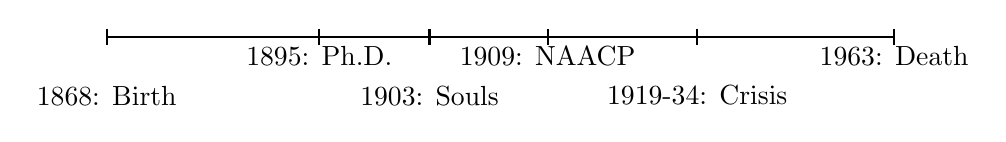
\begin{tikzpicture}
				\draw[thick, -] (0,0) -- (10,0);
				\node[below] at (0,-0.5) {1868: Birth};
				\node[below] at (2.7,0) {1895: Ph.D.};
				\node[below] at (4.1,-0.5) {1903: Souls};
				\node[below] at (5.6,0) {1909: NAACP};
				\node[below] at (7.5,-0.5) {1919-34: Crisis};
				\node[below] at (10,0) {1963: Death};
				
				\foreach \x in {0,2.7,4.1,5.6,7.5,10} {
					\draw[thick] (\x,0.1) -- (\x,-0.1);
				}
			\end{tikzpicture}
		\end{center}
		
	\end{frame}
	
	% Slide 12: Du Bois vs. Washington
	\begin{frame}
		\frametitle{Du Bois vs. Washington: Competing Visions for Progress}
		
		\begin{itemize}
			\item Du Bois directly challenged Booker T. Washington's approach to racial advancement outlined in the Atlanta Compromise (1895).
			\item \textbf{Washington's philosophy} emphasized vocational education, economic self-sufficiency, and accommodating to white power structures.
			\item \textbf{Du Bois's approach} demanded full political rights, higher education, and direct confrontation with discrimination.
			\item This debate represented contrasting ethical assessments of how to respond to injustice—accommodation versus resistance.
		\end{itemize}
		
		\begin{columns}
			\column{0.48\textwidth}
			\textbf{Washington's Position}
			\begin{itemize}
				\item Economic independence first
				\item Industrial education
				\item Gradual, indirect approach
				\item Acceptance of segregation
			\end{itemize}
			
			\column{0.48\textwidth}
			\textbf{Du Bois's Critique}
			\begin{itemize}
				\item Political rights essential
				\item Liberal arts education
				\item Immediate equality
				\item Challenge to segregation
			\end{itemize}
		\end{columns}
		
	\end{frame}
	
	% Slide 13: The Talented Tenth
	\begin{frame}
		\frametitle{The Talented Tenth: Education and Leadership Philosophy}
		
		\begin{itemize}
			\item In his 1903 essay, Du Bois argued that the \textbf{Talented Tenth}—highly educated Black Americans—should lead racial advancement.
			\item This educated elite would serve as teachers, writers, and leaders who could articulate rights claims and guide progress.
			\item Du Bois believed liberal arts education, not just vocational training, was necessary for developing effective leadership.
			\item The concept reflects a tension between meritocracy and collective uplift in Du Bois's early thought.
		\end{itemize}
		
		\begin{exampleblock}{Du Bois on the Talented Tenth}
			"The Negro race, like all races, is going to be saved by its exceptional men. The problem of education, then, among Negroes must first of all deal with the Talented Tenth; it is the problem of developing the Best of this race that they may guide the Mass away from the contamination and death of the Worst."
		\end{exampleblock}
		
	\end{frame}
	
	% Slide 14: The Veil and Double Consciousness
	\begin{frame}
		\frametitle{The Veil and Double Consciousness: Living Behind the Color Line}
		
		\begin{itemize}
			\item In \textit{The Souls of Black Folk} (1903), Du Bois introduces the concept of the \textbf{Veil} as a metaphor for racial separation.
			\item The Veil represents the physical and psychological barrier between Black and white Americans.
			\item \textbf{Double consciousness} describes the "sense of always looking at one's self through the eyes of others."
			\item These concepts illuminate the psychological and ethical dimensions of living under racism.
		\end{itemize}
		
		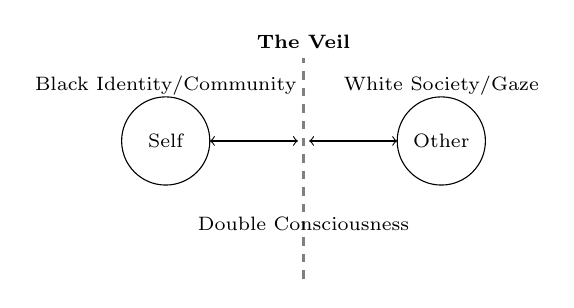
\begin{tikzpicture}[scale=0.7]
			\scriptsize
			% Draw the veil
			\draw[thick, dashed, gray] (5,0) -- (5,4);
			\node at (5,4.3) {\textbf{The Veil}};
			
			% Left side - Black identity
			\node at (2.5,3.5) {Black Identity/Community};
			\draw (2.5,2.5) circle (0.8) node {Self};
			
			% Right side - White society
			\node at (7.5,3.5) {White Society/Gaze};
			\draw (7.5,2.5) circle (0.8) node {Other};
			
			% Double consciousness arrows
			\draw[<->] (3.3,2.5) -- (4.9,2.5);
			\draw[<->] (5.1,2.5) -- (6.7,2.5);
			
			% Label
			\node at (5,1) {Double Consciousness};
		\end{tikzpicture}
		
	\end{frame}
	
	% Slide 15: Psychological Wages of Whiteness
	\begin{frame}
		\frametitle{Psychological Wages of Whiteness: Understanding Privilege}
		
		\begin{itemize}
			\item In \textit{Black Reconstruction in America} (1935), Du Bois developed the concept of the \textbf{psychological wage} of whiteness.
			\item This "public and psychological wage" compensated poor whites for their economic exploitation with racial status.
			\item The concept explains how white workers often prioritized racial advantages over class solidarity.
			\item This analysis reveals how racial hierarchy functions to preserve economic power structures.
		\end{itemize}
		
		\begin{block}{Key Insight}
			"It must be remembered that the white group of laborers, while they received a low wage, were compensated in part by a sort of public and psychological wage. They were given public deference and titles of courtesy because they were white."
		\end{block}
		
	\end{frame}
	
	% Slide 16: Du Bois's Critique of American Democracy
	\begin{frame}
		\frametitle{Du Bois's Critique of American Democracy}
		
		\begin{itemize}
			\item Du Bois argued that American democracy failed to fulfill its promises for Black Americans.
			\item He identified racism as a fundamental contradiction within American democratic ideals.
			\item Du Bois challenged liberal assumptions that gradual progress would inevitably resolve racial injustice.
			\item His critique questioned whether American democracy could achieve justice without confronting white supremacy.
		\end{itemize}
		
		\begin{table}
			\begin{tabular}{ll}
				\toprule
				\textbf{Democratic Promises} & \textbf{Contradictory Realities} \\
				\midrule
				Equal citizenship & Disenfranchisement \\
				Equal protection & Lynch law and violence \\
				Economic opportunity & Labor discrimination \\
				Political representation & Exclusion from governance \\
				\bottomrule
			\end{tabular}
		\end{table}
		
	\end{frame}
	
	% Slide 17: Du Bois's Evolving Thought
	\begin{frame}
		\frametitle{Du Bois's Evolving Thought on Race and Justice}
		
		\begin{itemize}
			\item Over his long career, Du Bois's thinking evolved from liberal reformism to more radical critiques of capitalism and colonialism.
			\item He increasingly connected racial oppression in America to global colonialism and economic exploitation.
			\item In his later years, Du Bois embraced \textbf{Pan-Africanism}, the idea that people of African descent worldwide share common interests.
			\item He died in Ghana in 1963, having renounced his American citizenship and embraced a more international perspective on racial justice.
		\end{itemize}
		
		\begin{center}
			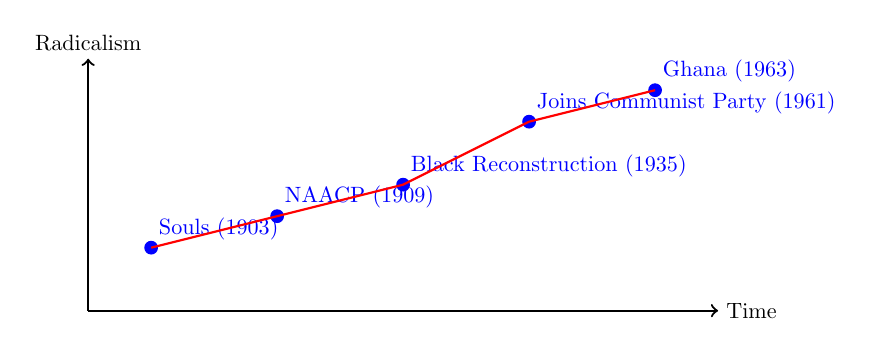
\begin{tikzpicture}[scale=0.8, every node/.style={scale=0.8}]
				\draw[->, thick] (0,0) -- (10,0) node[right] {Time};
				\draw[->, thick] (0,0) -- (0,4) node[above] {Radicalism};
				
				% Position points on the timeline
				\filldraw[blue] (1,1) circle (0.1) node[above right] {Souls (1903)};
				\filldraw[blue] (3,1.5) circle (0.1) node[above right] {NAACP (1909)};
				\filldraw[blue] (5,2) circle (0.1) node[above right] {Black Reconstruction (1935)};
				\filldraw[blue] (7,3) circle (0.1) node[above right] {Joins Communist Party (1961)};
				\filldraw[blue] (9,3.5) circle (0.1) node[above right] {Ghana (1963)};
				
				% Draw path of evolution
				\draw[red, thick] (1,1) -- (3,1.5) -- (5,2) -- (7,3) -- (9,3.5);
			\end{tikzpicture}
		\end{center}
		
	\end{frame}
	
	% Slide 18: Martin Luther King Jr.
	\begin{frame}
		\frametitle{Martin Luther King Jr.: Intellectual and Spiritual Foundations}
		
		\begin{itemize}
			\item Martin Luther King Jr. (1929-1968) emerged as a leader during the Montgomery Bus Boycott (1955-56).
			\item King's philosophy combined \textbf{Christian theology}, specifically the Social Gospel tradition, with democratic ideals.
			\item He studied the works of Mohandas Gandhi and developed a philosophy of nonviolent direct action.
			\item King's doctorate in systematic theology from Boston University shaped his intellectual approach to justice.
		\end{itemize}
		
		\begin{block}{King's Intellectual Influences}
			\scriptsize
			\begin{itemize}
				\item \textbf{Religious}: Jesus Christ, Walter Rauschenbusch's Social Gospel
				\item \textbf{Philosophical}: Personalism, Hegel's dialectic
				\item \textbf{Political}: Gandhi's nonviolence, Henry David Thoreau's civil disobedience
				\item \textbf{Black Tradition}: Howard Thurman, Benjamin Mays
			\end{itemize}
		\end{block}
		
	\end{frame}
	
	% Slide 19: King's Critique of the White Moderate
	\begin{frame}
		\frametitle{King's Critique of the White Moderate: The Ethics of Neutrality}
		
		\begin{itemize}
			\item In "Letter from Birmingham Jail" (1963), King criticized the \textbf{white moderate} who prefers "order" over justice.
			\item King argued that moderates' commitment to gradualism enabled continued injustice.
			\item He identified moral neutrality in the face of oppression as a form of complicity.
			\item This critique challenged the ethical stance that patience and compromise were adequate responses to injustice.
		\end{itemize}
		
		\begin{exampleblock}{King on the White Moderate}
			"I have almost reached the regrettable conclusion that the Negro's great stumbling block in his stride toward freedom is not the White Citizen's Counciler or the Ku Klux Klanner, but the white moderate, who is more devoted to 'order' than to justice; who prefers a negative peace which is the absence of tension to a positive peace which is the presence of justice."
		\end{exampleblock}
		
	\end{frame}
	
	% Slide 20: Civil Disobedience
	\begin{frame}
		\frametitle{When is Civil Disobedience Justified? King's Framework}
		
		\begin{itemize}
			\item King developed a sophisticated framework for \textbf{civil disobedience} as a moral response to unjust laws.
			\item He distinguished between just laws that uphold human dignity and unjust laws that degrade human personality.
			\item Civil disobedience requires willingness to accept consequences, demonstrating respect for law as a concept.
			\item King's approach balanced moral absolutes with practical considerations about effective resistance.
		\end{itemize}
		
		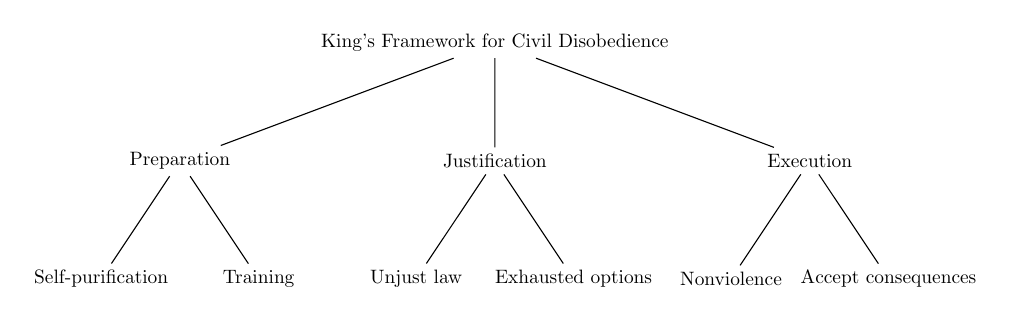
\begin{tikzpicture}[
			level 1/.style={sibling distance=40mm},
			level 2/.style={sibling distance=20mm},
			every node/.style={scale=0.7}
			]
			\node {King's Framework for Civil Disobedience}
			child {node {Preparation}
				child {node {Self-purification}}
				child {node {Training}}
			}
			child {node {Justification}
				child {node {Unjust law}}
				child {node {Exhausted options}}
			}
			child {node {Execution}
				child {node {Nonviolence}}
				child {node {Accept consequences}}
			};
		\end{tikzpicture}
		
	\end{frame}
	
	% Slide 21: The Beloved Community
	\begin{frame}
		\frametitle{The Beloved Community: King's Vision of Social Harmony}
		
		\begin{itemize}
			\item King envisioned the \textbf{Beloved Community} as the ultimate goal of the civil rights movement.
			\item This concept described a society based on justice, equal opportunity, and love for fellow human beings.
			\item The Beloved Community would transcend racism through reconciliation rather than victory of one group over another.
			\item This vision reflected King's belief that human destiny is shared and interconnected.
		\end{itemize}
		
		\begin{center}
			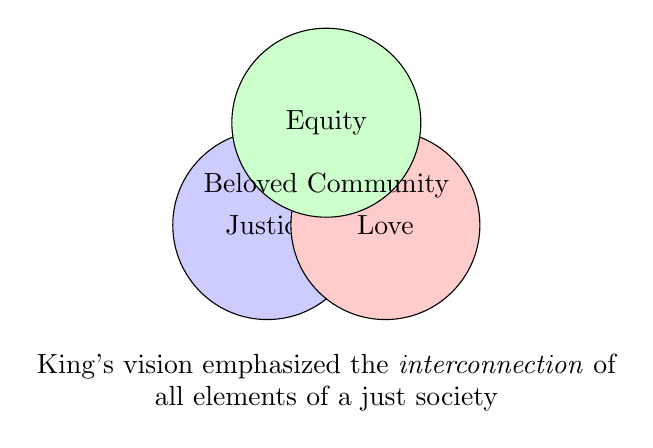
\begin{tikzpicture}
				% Draw overlapping circles representing interconnected community
				\draw[fill=blue!20] (0,0) circle (1.2) node {Justice};
				\draw[fill=red!20] (1.5,0) circle (1.2) node {Love};
				\draw[fill=green!20] (0.75,1.3) circle (1.2) node {Equity};
				
				% Label the intersection
				\node at (0.75,0.5) {Beloved Community};
				
				% Add caption
				\node at (0.75,-1.8) {King's vision emphasized the \textit{interconnection} of};
				\node at (0.75,-2.2) {all elements of a just society};
			\end{tikzpicture}
		\end{center}
		
	\end{frame}
	
	% Slide 22: The Triple Evils
	\begin{frame}
		\frametitle{The Triple Evils: Racism, Poverty, and War as Interconnected Injustices}
		
		\begin{itemize}
			\item King identified the \textbf{Triple Evils} of racism, poverty, and militarism as interconnected social problems.
			\item He argued that these issues reinforce each other and require comprehensive solutions.
			\item This analysis expanded King's focus beyond civil rights to economic justice and opposition to the Vietnam War.
			\item The Triple Evils framework challenged the separation of domestic and international ethical concerns.
		\end{itemize}
		
		\begin{table}
			\begin{tabular}{lll}
				\toprule
				\textbf{Evil} & \textbf{Manifestation} & \textbf{Moral Challenge} \\
				\midrule
				Racism & Segregation, discrimination & Dignity and equality \\
				Poverty & Economic exploitation & Material justice \\
				Militarism & Vietnam War, arms race & Peace and nonviolence \\
				\bottomrule
			\end{tabular}
		\end{table}
		
	\end{frame}
	
	% Slide 23: King's Philosophy of Nonviolence
	\begin{frame}
		\frametitle{King's Philosophy of Nonviolence: Principles and Practices}
		
		\begin{itemize}
			\item King's philosophy of \textbf{nonviolence} went beyond tactical considerations to ethical principles about human relationships.
			\item Nonviolence seeks to defeat injustice, not to defeat or humiliate opponents.
			\item The approach requires willingness to accept suffering without retaliation, transforming pain into social progress.
			\item King believed nonviolence had transformative power for practitioners and witnesses alike.
		\end{itemize}
		
		\begin{block}{Six Principles of Nonviolence}
			\scriptsize
			\begin{enumerate}
				\item Nonviolence is a way of life for courageous people
				\item Nonviolence seeks to win friendship and understanding
				\item Nonviolence seeks to defeat injustice, not people
				\item Nonviolence holds that suffering can educate and transform
				\item Nonviolence chooses love instead of hate
				\item Nonviolence believes the universe is on the side of justice
			\end{enumerate}
		\end{block}
		
	\end{frame}
	
	% Slide 24: King's Expanding Vision
	\begin{frame}
		\frametitle{From Civil Rights to Human Rights: King's Expanding Vision}
		
		\begin{itemize}
			\item In his later years, King expanded his focus from civil rights to \textbf{human rights} and economic justice.
			\item The Poor People's Campaign (1968) sought to address poverty across racial lines through economic restructuring.
			\item King increasingly criticized capitalism and militarism as systems that perpetuated injustice.
			\item This expanded vision connected domestic civil rights with international human rights struggles.
		\end{itemize}
		
		\begin{alertblock}{King's Later Vision}
			"True compassion is more than flinging a coin to a beggar. It comes to see that an edifice which produces beggars needs restructuring."
		\end{alertblock}
		
	\end{frame}
	
	% Slide 25: Kwame Anthony Appiah
	\begin{frame}
		\frametitle{Kwame Anthony Appiah: Philosophical Background and Influences}
		
		\begin{itemize}
			\item Kwame Anthony Appiah (born 1954) is a gay Ghanaian-British-American philosopher who addresses race, identity, and ethics.
			\item His multicultural background—British mother and Ghanaian father—informs his philosophical perspective.
			\item Appiah synthesizes analytic philosophy with cross-cultural insights and historical analysis.
			\item His work builds on and critically engages with earlier philosophers while addressing contemporary ethical concerns.
		\end{itemize}
		
		\begin{block}{Major Works on Race and Ethics}
			\scriptsize
			\begin{itemize}
				\item \textit{In My Father's House} (1992)
				\item \textit{Color Conscious} (with Amy Gutmann, 1996)
				\item \textit{The Ethics of Identity} (2005)
				\item \textit{Cosmopolitanism: Ethics in a World of Strangers} (2006)
				\item \textit{The Lies That Bind: Rethinking Identity} (2018)
			\end{itemize}
		\end{block}
		
	\end{frame}
	
	% Slide 26: Racial Anti-Realism
	\begin{frame}
		\frametitle{Racial Anti-Realism: Challenging Biological Conceptions of Race}
		
		\begin{itemize}
			\item Appiah's \textbf{racial anti-realism} argues that race as understood in biological terms does not meaningfully exist.
			\item He demonstrates that genetic variation within supposed "racial" groups exceeds variation between such groups.
			\item Appiah distinguishes between biological race (which he rejects) and racial identity (which he acknowledges as socially real).
			\item This position challenges both racist ideologies and certain forms of identity politics.
		\end{itemize}
		
		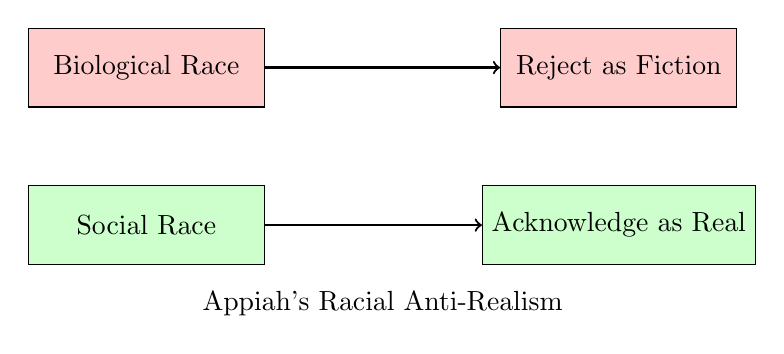
\begin{tikzpicture}
			% Diagram showing the relationship between concepts
			\node[draw, rectangle, fill=red!20, minimum width=3cm, minimum height=1cm] (biological) at (0,2) {Biological Race};
			\node[draw, rectangle, fill=green!20, minimum width=3cm, minimum height=1cm] (social) at (0,0) {Social Race};
			
			\node[draw, rectangle, fill=red!20, minimum width=3cm, minimum height=1cm] (rejection) at (6,2) {Reject as Fiction};
			\node[draw, rectangle, fill=green!20, minimum width=3cm, minimum height=1cm] (acknowledge) at (6,0) {Acknowledge as Real};
			
			\draw[->, thick] (biological) -- (rejection);
			\draw[->, thick] (social) -- (acknowledge);
			
			\node at (3,-1) {Appiah's Racial Anti-Realism};
		\end{tikzpicture}
		
	\end{frame}
	
	% Slide 27: Racial Anti-Realism Implications
	\begin{frame}
		\frametitle{Racial Anti-Realism: Social and Ethical Implications}
		
		\begin{itemize}
			\item Appiah argues that biological race concepts often serve as pseudoscientific justifications for oppression.
			\item The social construction of race has real-world consequences in shaping identities and distributing resources.
			\item Racial anti-realism does not deny racism's effects but reframes how we understand and address racial injustice.
			\item This view leads to a more nuanced approach to racial identity as historically contingent rather than essential.
		\end{itemize}
		
		\begin{exampleblock}{Appiah on Racial Categories}
			"The truth is that there are no races: there is nothing in the world that can do all we ask race to do for us... The evil that is done is done by the concept, and by easy—yet impossible—assumptions about its application."
		\end{exampleblock}
		
	\end{frame}
	
	% Slide 28: Cosmopolitanism
	\begin{frame}
		\frametitle{Cosmopolitanism: Ethics in a World of Strangers}
		
		\begin{itemize}
			\item \textbf{Cosmopolitanism} in Appiah's framework combines universal concern for all human beings with respect for legitimate differences.
			\item He rejects both rigid universalism that ignores cultural specificity and relativism that abandons shared ethical standards.
			\item Cosmopolitan ethics acknowledges the value of particular cultural traditions while maintaining cross-cultural dialogue.
			\item This approach seeks to balance universal human rights with respect for diverse ways of life.
		\end{itemize}
		
		\begin{table}
			\begin{tabular}{lll}
				\toprule
				\textbf{Position} & \textbf{Universal Values} & \textbf{Cultural Differences} \\
				\midrule
				Universalism & Embraced & Ignored/Minimized \\
				Relativism & Rejected & Absolutized \\
				\textbf{Cosmopolitanism} & \textbf{Core values affirmed} & \textbf{Respected within limits} \\
				\bottomrule
			\end{tabular}
		\end{table}
		
	\end{frame}
	% Slide 29: Cosmopolitanism Continued
	\begin{frame}
		\frametitle{Cosmopolitanism: Universal Ethical Principles Across Cultural Differences}
		
		\begin{itemize}
			\item Appiah's cosmopolitanism emphasizes \textbf{conversation} across differences as essential to ethical progress.
			\item He argues that moral disagreements can be productive without requiring complete consensus.
			\item Cosmopolitanism acknowledges that people have obligations to those beyond their immediate communities.
			\item This approach seeks a middle path between imperialist universalism and isolationist particularism.
		\end{itemize}
		
		\begin{center}
			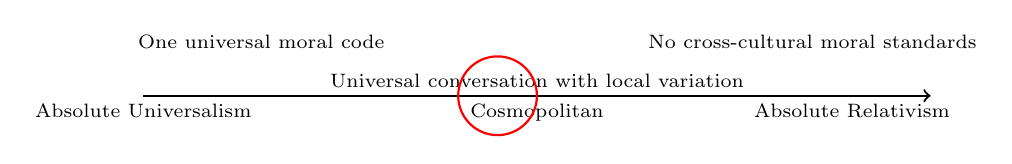
\begin{tikzpicture}
				\scriptsize
				% Create a spectrum with positions
				\draw[thick, ->] (0,0) -- (10,0);
				\node[below] at (0,0) {Absolute Universalism};
				\node[below] at (9,0) {Absolute Relativism};
				\node[below, text width=3cm, align=center] at (5,0) {Cosmopolitan};
				
				% Add examples
				\node[above] at (1.5,0.5) {One universal moral code};
				\node[above] at (5,0) {Universal conversation with local variation};
				\node[above] at (8.5,0.5) {No cross-cultural moral standards};
				
				% Mark Appiah's position
				\draw[red, thick] (4.5,0) circle (0.5);
			\end{tikzpicture}
		\end{center}
		
	\end{frame}
	
	% Slide 30: Identity Construction
	\begin{frame}
		\frametitle{Identity: Virtue Ethics and Authentic Self-Development}
		
		\begin{itemize}
			\item Appiah analyzes identity as both socially constructed and individually negotiated through ethical choices.
			\item \textbf{Identities} provide scripts that shape our understanding of how to live but don't determine our actions.
			\item He explores the ethics of authentic self-development within inherited identity categories.
			\item This approach examines how people can reshape collective identities through their individual ethical choices.
		\end{itemize}
		
		\begin{block}{Appiah on Identity Construction}
			"Identities are complex and multiple and grow out of a history of changing responses to economic, political, and cultural forces, almost always in opposition to other identities... They flourish despite our ignorance of their origins, despite the misunderstandings that form them."
		\end{block}
		
	\end{frame}
	
	% Slide 31: Identity Continued
	\begin{frame}
		\frametitle{Identity: Negotiating Multiple Social Categories}
		
		\begin{itemize}
			\item Appiah challenges \textbf{essentialism}—the idea that identities have fixed, inherent characteristics.
			\item He emphasizes that all people navigate multiple, overlapping identities simultaneously.
			\item Real ethical freedom requires acknowledging the contingency of identity categories.
			\item This view frames identity as narrative and dialogical rather than predetermined or static.
		\end{itemize}
		
		\begin{center}
			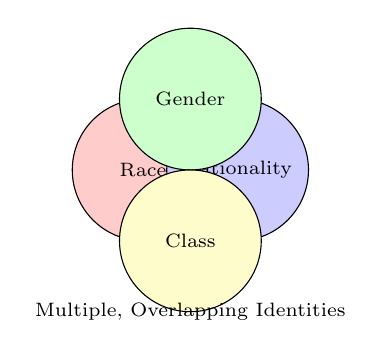
\begin{tikzpicture}[scale=.6]
				\scriptsize
				% Create overlapping circles for different identity dimensions
				\draw[fill=red!20] (0,0) circle (1.5) node {Race};
				\draw[fill=blue!20] (2,0) circle (1.5) node {Nationality};
				\draw[fill=green!20] (1,1.5) circle (1.5) node {Gender};
				\draw[fill=yellow!20] (1,-1.5) circle (1.5) node {Class};
				
				
				% Add title
				\node at (1,-3) {Multiple, Overlapping Identities};
			\end{tikzpicture}
		\end{center}
		
	\end{frame}
	
	% Slide 32: Appiah's Challenge
	\begin{frame}
		\frametitle{Appiah's Challenge to Racial Thinking in Contemporary Ethics}
		
		\begin{itemize}
			\item Appiah argues that ethical progress requires moving beyond racial essentialist thinking while acknowledging racism's effects.
			\item He challenges both color-blind approaches that ignore ongoing injustice and rigid identity politics that reinforce racial divisions.
			\item Appiah encourages ethical engagement with history without being determined by it.
			\item This balanced approach seeks to address real injustices while avoiding reification of problematic categories.
		\end{itemize}
		
		\begin{columns}
			\column{0.48\textwidth}
			\textbf{What Appiah Rejects}
			\begin{itemize}
				\item Biological race
				\item Racial essentialism
				\item Uncritical identity politics
				\item Cultural isolationism
			\end{itemize}
			
			\column{0.48\textwidth}
			\textbf{What Appiah Affirms}
			\begin{itemize}
				\item Social reality of race
				\item Historical analysis of racism
				\item Cross-cultural dialogue
				\item Cosmopolitan ethics
			\end{itemize}
		\end{columns}
		
	\end{frame}
	
	% Slide 33: Connecting Historical and Contemporary Approaches
	\begin{frame}
		\frametitle{Connecting Historical and Contemporary Approaches to Race and Ethics}
		
		\begin{itemize}
			\item The philosophers we've studied share concerns with human dignity, freedom, and ethical consistency.
			\item Their approaches evolved in response to changing historical conditions and intellectual developments.
			\item Du Bois, King, and Appiah each developed frameworks that combined ethical theory with practical engagement.
			\item Understanding these thinkers in relation to each other reveals the evolving nature of ethical thinking about race.
		\end{itemize}
		
		\begin{center}
			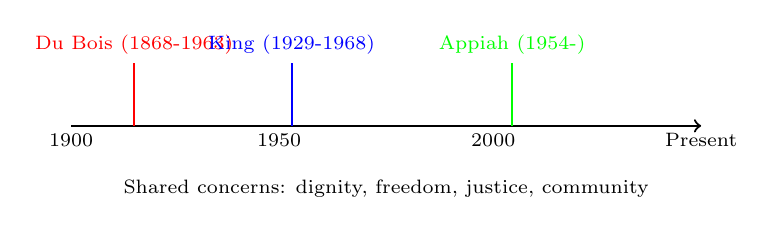
\begin{tikzpicture}[scale=0.8]
				\scriptsize
				% Timeline with key figures
				\draw[thick, ->] (0,0) -- (10,0);
				\node[below] at (0,0) {1900};
				\node[below] at (3.3,0) {1950};
				\node[below] at (6.7,0) {2000};
				\node[below] at (10,0) {Present};
				
				% Key figures
				\draw[red, thick] (1,0) -- (1,1) node[above] {Du Bois (1868-1963)};
				\draw[blue, thick] (3.5,0) -- (3.5,1) node[above] {King (1929-1968)};
				\draw[green, thick] (7,0) -- (7,1) node[above] {Appiah (1954-)};
				
				% Shared concerns
				\node at (5,-1) {Shared concerns: dignity, freedom, justice, community};
			\end{tikzpicture}
		\end{center}
		
	\end{frame}
	
	% Slide 34: Contemporary Applications
	\begin{frame}
		\frametitle{Applying Ethical Insights to Contemporary Racial Justice Issues}
		
		\begin{itemize}
			\item The insights of these philosophers provide frameworks for addressing contemporary ethical challenges.
			\item Du Bois's analysis of structural disadvantage remains relevant to understanding persistent racial inequalities.
			\item King's nonviolent ethics offers guidance for social movements seeking justice through moral means.
			\item Appiah's critique of essentialism provides tools for navigating complex identity politics in diverse societies.
		\end{itemize}
		
		\begin{table}
			\begin{tabular}{lll}
				\toprule
				\textbf{Contemporary Issue} & \textbf{Relevant Philosopher} & \textbf{Key Concept} \\
				\midrule
				Persistent inequality & Du Bois & Structural analysis \\
				Protest movements & King & Nonviolent resistance \\
				Identity politics & Appiah & Anti-essentialism \\
				Global justice & All three & Different approaches \\
				\bottomrule
			\end{tabular}
		\end{table}
		
	\end{frame}
	
	% Slide 35: Discussion Questions I
	\begin{frame}
		\frametitle{Discussion Questions I}
		
		\begin{exampleblock}{Questions on Historical Foundations and Du Bois}
			\begin{itemize}
				\item How did abolitionists articulate moral arguments against slavery, and how did these arguments engage with American founding principles?
				\item Is Washington's accommodationist approach to racial progress inherently compromised, or does it represent a legitimate ethical strategy given historical constraints?
				\item How does Du Bois's concept of "double consciousness" reveal ethical challenges faced by marginalized groups navigating majority cultures?
				\item In what ways does the concept of the "psychological wage of whiteness" help explain the persistence of racism despite apparent economic disadvantages for some white communities?
			\end{itemize}
		\end{exampleblock}
		
	\end{frame}
	
	% Slide 36: Discussion Questions II
	\begin{frame}
		\frametitle{Discussion Questions II}
		
		\begin{exampleblock}{Questions on King, Appiah, and Contemporary Applications}
			\begin{itemize}
				\item What are the ethical implications of King's critique of the "white moderate," and how might this critique apply to contemporary issues?
				\item How does King justify civil disobedience as a moral action while still respecting the rule of law as a concept?
				\item How does Appiah's racial anti-realism challenge our ethical thinking without undermining the need to address historical and ongoing racial injustice?
				\item What moral responsibilities toward others might follow from Appiah's cosmopolitan framework, and how do these compare with King's Beloved Community?
			\end{itemize}
		\end{exampleblock}
		
	\end{frame}
	
\end{document}